\subsection{先行研究における特異型EEJのレビュー}
\label{sec:review_peculiar_eej}

特異型EEJに関する先行研究として、池末 (2024) \cite{Ikesue2024} による調査が挙げられる。


同研究では、2014年から2020年の期間におけるMAGDAS観測網のデータを用いた解析が行われた。
解析対象の観測点として、ペルー領域のANC, HUA, EUSが使用された。
また、地磁気静穏時のイベントを抽出するために、Kp指数が4未満 ($Kp < 4$)、かつ赤道擾乱指数 (EDst) が-30 nTより大きい ($EDst > -30$ nT) という条件が適用された。

特異型EEJの分類方法として下記のように*目視*で分類した(figure:ikesue_peculiar_type)
1: 未発達型
dip観測点においてEEJが発達しておらず,offdip観測点のEUELと同程度の形状を示す
2: 突発型
    EEJが本来卓越する時間帯(12:00LT)で大きな落ち込みを見せる形状
    特にdip観測点のピークが0nT以下になるものを**CEJ型**、0nT以上になるものを**急落型**と定義した
3: その他型
    上記した型に当てはまらなく大きく乱れている形状

\begin{figure}[htbp]
  \centering
  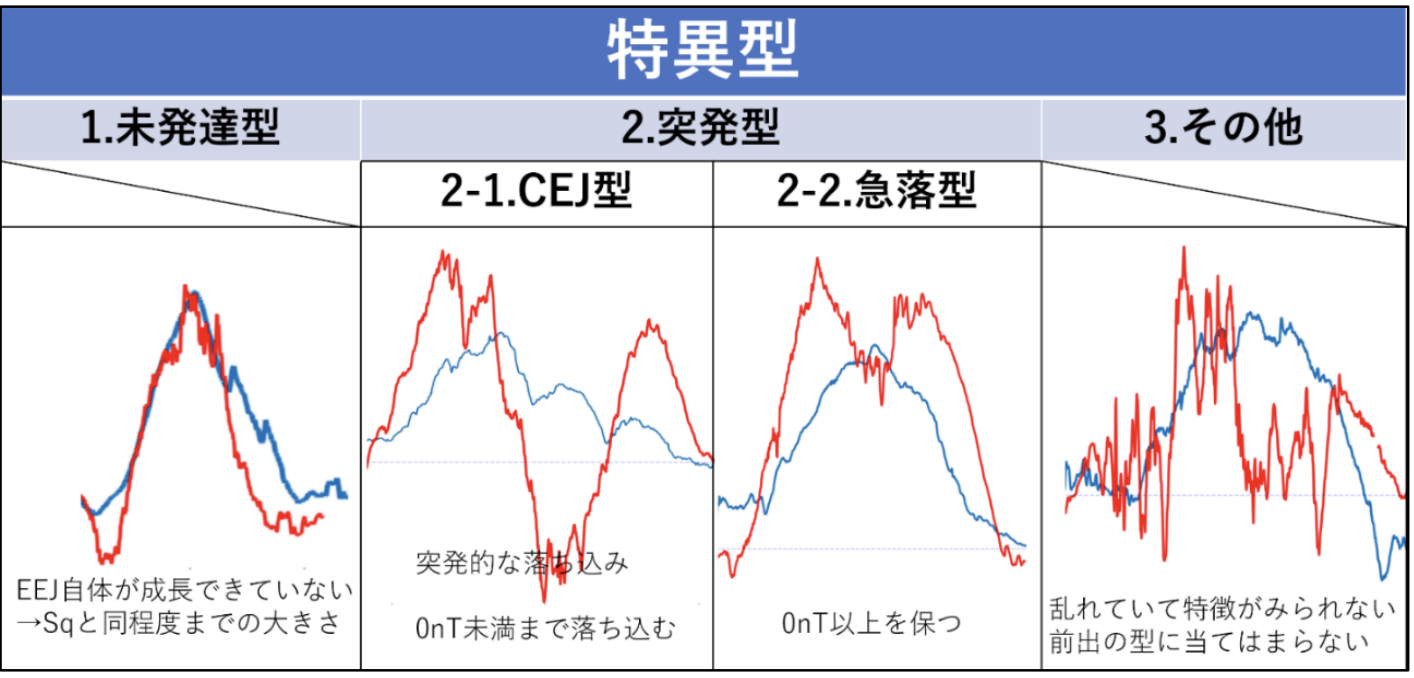
\includegraphics[width=\linewidth]{figures/ikesue_peculiar_type.png}
  \caption{特異型EEJの分類 (\citeauthor{Ikesue2024}\citetype{Ikesue2024}より引用)}
  \label{fig:ikesue_peculiar_type}
\end{figure}

特に、未発達型の発生数の季節変動を調査したところ、夏季（11〜1月）に発生数が多くなる傾向が確認された（図 \ref{fig:ikesue_undeveloped}）。
また、月潮汐効果の対応関係を調査したところDip観測点で西向き電流が流れる期間に突発型が多く発生しやすいことが示唆されていた。


\begin{figure}[htbp]
  \centering
  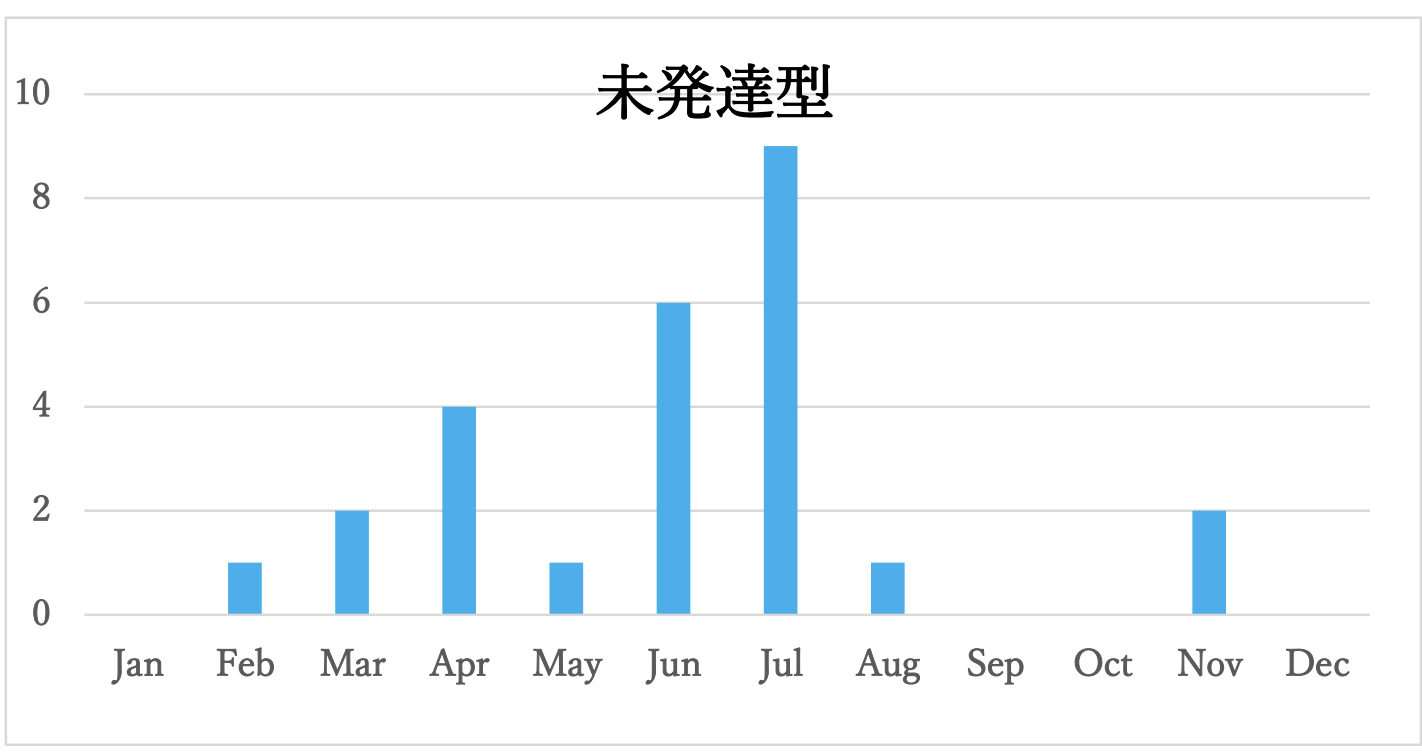
\includegraphics[width=\linewidth]{figures/ikesue_undeveloped.png}
  \caption{未発達型の季節変化 (\citeauthor{Ikesue2024}\citetype{Ikesue2024}より引用)}
  \label{fig:ikesue_undeveloped}
\end{figure}